%!TEX encoding = UTF8
%!TEX root = 0-notes.tex

\chapter{Suites}

\section{Introduction}

\dfn{Suite}{
	On appelle \emph{suite} une fonction $u$ réelle prenant des entiers naturels $n\in\N$.
	
	Le \emph{terme initial} de la suite est donné par $u(0)$.
	Le \emph{terme de rang $n$} de la suite est donné par $u(n)$.
}{dfn:suite}

\nt{
	Une suite est une liste de valeurs réelles $u(0), u(1), u(2), \dots$.
	On peut connaitre tous les termes d'une suite dès qu'elle est définie \emph{algébriquement}.
	C'est-à-dire, si $u(n) = \big(\text{expression en fonction de $n$}\big)$ pour tout $n\in\N$.
}

\ex{}{
	La suite donnée algébriquement par $u(n) = n-1$ pour tout $n\in\N$ est entièrement connue.
	Son terme initial est $u(0) = -1$, et son terme de rang $210$ est $u(210) = 209$.
}{ex:suite-alg}

\ex{}{
	Les fonctions suivantes sont des suites données par leur rang $n$ : on connait donc leur valeur pour tout les entiers naturels.
	\begin{multicols}{2}
	\begin{enumerate}
		\item $u(n) = n+1$
		\item $v(n) = n^2$
		\item $\xi(n) = \dfrac1{n^3}$
		\item $a(n) = (n+1)^n$
	\end{enumerate}
	\end{multicols}
	Une suite n'a pas forcément de formule générale pour tout $n$, c'est une simplement \emph{suite} de nombres réels.
}{}

\nt{
	Certaines suites peuvent être définies \emph{récursivement}.
	Le terme de rang $n$ dépendra des termes de rangs inférieurs.
}

\ex{}{
	Considérons la suite $u$ de terme initial $u(0) = 0$ et vérifiant, pour tout $n\in\N$,
		\[ u(n+1) = u(n) + 2. \]
	On lit « le terme de rang $n+1$ est égal au terme de rang $n$ plus 2 » ou, autrement dit, « pour passer d'un terme au suivant, il faut ajouter 2 ».
	Ainsi $u(1) = u(0) + 2 = 2, u(2) = 4, u(3) = 6, \dots$.
	
	Pour calculer $u(341)$, il faut, \emph{a priori} nécessairement calculer tous les termes de rang inférieur à $341$.
	Cependant, il semblerait $u(n) = 2n$ pour tout $n\in\N$, et donc qu'on ait immédiatement $u(341) = 682$.
}{ex:suite-rec}

\section{Suites arithmétiques}

\subsection{Introduction}

\dfn{Suite arithmétique}{
	Une suite arithmétique $u$ est une suite vérifiant, pour tout $n\in\N$,
		\[ u(n+1) = u(n) + a, \]
	où $a\in\R$ est un nombre fixé qu'on appelle la \emph{raison}.
	
	On lit :
		\begin{center}
			« Pour passer d'un terme au suivant, on ajoute la raison $a$. »
		\end{center}
}{dfn:suite-arithmetique}

\exe{}{
	Donner les 5 premiers termes de la suite arithmétique $u$ de raison 1 et de terme initial $u(0) = 0$.
	Faire une conjecture sur l'expression algébrique de $u(n)$ pour tout $n\in\N$.
}{exe:arithm1}{
	Pour passer d'un rang au suivant, on ajoute la raison, ici $1$.
	Donc $u(1) = 0+1=1, u(2) = 2, u(3) = 3, u(4) = 4$.
	
	Il semblerait que $u(n) = n$ pour tout $n\in\N$.
}

\exe{}{
	Donner les 5 premiers termes de la suite arithmétique $v$ de raison 1 et de terme initial $v(0) = 3$.
	Faire une conjecture sur l'expression algébrique de $u(n)$.
}{exe:arithm2}{
	Pour passer d'un rang au suivant, on ajoute la raison, ici $1$.
	Donc $v(1) = 3+1=4, v(2) = 5, v(3) = 6, v(4) = 7$.
	
	Il semblerait que $v(n) = n+1$ pour tout $n\in\N$.
}

\exe{}{
	Donner les 5 premiers termes de la suite arithmétique $w$ de raison -5 et de terme initial $w(0) = 5$.
	Faire une conjecture sur l'expression algébrique de $u(n)$.
}{exe:arithm3}{
	Pour passer d'un rang au suivant, on ajoute la raison, ici $-5$.
	Donc $w(1) = 5-5=0, w(2) = -5, w(3) = -10, w(4) = -15$.
	
	Il semblerait que $w(n) = -5(n-1) = -5n + 5$ pour tout $n\in\N$.
}

\exe{}{
	Montrer que la suite $u$ dont les trois premiers termes sont $u(0) = 3, u(1) = 10, u(2) = 20$ ne peut pas être arithmétique.
}{exe:nonarithm}{
	Pour passer d'un terme au suivant, on ajoute $7$ puis $10$.
	Si $u$ était arithmétique, on aurait ajouté la même quantité (sa raison). \Large\Lightning
}

\exe{}{
	Montrer que la suite $v$ telle que $v(41) = -10, v(42) = -20, v(44) = -30$ ne peut pas être arithmétique.
}{exe:nonarithm2}{
	Si $v$ était arithmétique, sa raison serait $-10$ car c'est ce qu'on ajoute pour passer du terme 41 au terme 42.
	Cependant, dans ce cas, on aurait $v(43) = -30$ et $v(44) = -40$, ce qui est contradictoire avec la donnée de l'exercice. \Large\Lightning
}

\exe{, difficulty=1}{
	Si une suite $w$ vérifie $w(10) = 1, w(11) = 3, w(12) = 5$, est-elle nécessairement arithmétique ?
}{exe:nonarithm3}{
	$w$ pourrait être arithmétique, auquel cas $w(n) = -9 + n$ pour tout $n\in\N$, mais ce n'est pas nécessairement le cas.
	On peut librement définir $w(13) = -100$ pour casser le caractère arithmétique de la suite. 
}

\exe{}{
	Soit $u$ une suite arithmétique de raison $7$ telle que $u(3) = 45$.
	Donner le terme initial de $u$.
}{exe:terme-initial}{
	Pour passer d'un rang au suivant, on doit ajouter $7$.
	Pour revenir en arrière d'un rang, on ajoute donc $-7$.
	Ainsi $u(2) = 45 - 7 = 38, u(1) = 38-7 = 31, u(0) = 31-7 = 24$.
}

\subsection{Expression algébrique}

\ex{}{
	La suite $u(n) = 2n$ est arithmétique de raison 2 car $u(n+1) = 2(n+1) = 2n + 2 = u(n) + 2$ pour tout $n\in\N$.
}{ex:suite-ar}

\exe{}{
	Montrer que la suite $u(n) = 7n+12$ est arithmétique. Donner sa raison et son terme initial.
}{exe:suite-ar}{
	La suite $u$ est arithmétique de raison 7 car $u(n+1) = 7(n+1) + 12 = 7n + 7 + 12 = (7n+12)+7 = u(n)+7$.
	Son terme initial est $u(0) = 12$.
}

\thm{}{
	Soit $u$ une suite arithmétique de raison $a$ et de terme initial $u(0)$.
	Alors, pour tout $n\in\N$,
		\[ u(n) = u(0) + n\cdot a. \]
}{thm:suite-arithmetique}

\pf{}{
	Pour passer du terme initial au suivant, $u(1)$, on ajoute $a$.
	Pour arriver à celui d'après, on ajoute à nouveau $a$.
	Donc pour arriver au $n$-ième terme, on doit ajoute $n$ fois $a$ : $u(n) = u(0) + n\cdot a$.
	Ceci est vrai pour n'importe quel $n\in\N$.
}

\exe{}{
	Donner l'expression algébrique de la suite $u$ définie récursivement comme suit.
		\[ \begin{cases*} u(0) = 3, \\ u(n+1) = u(n) - 1 & ($n\in\N$). \end{cases*}. \]
}{exe:arithm4}{
	$u$ est une suite arithmétique de terme initial $3$ et de raison $-1$.
	 D'après le théorème \ref{thm:suite-arithmetique}, $u(n) = 3-n$ pour tout $n\in\N$.
}

\subsection{Variations}

\mprop{Variations}{
	Soit $u$ une suite algébrique de raison $a$.
	On distingue alors les trois cas suivants.
		\begin{enumerate}[label=---]
			\item Si $a > 0$, alors $u$ est croissante linéairement.
			\item Si $a = 0$, alors $u$ est constante : $u(n) = u(0)$ pour tout $n\in\N$.
			\item Si $a < 0$, alors $u$ est décroissante linéairement.
		\end{enumerate}
}{}

\subsection{Sommes}

\exe{,difficulty=1}{
	On considère la série statistique $X=(0;1;2;\dots;19;20)$.
	Justifier sans calcul que la moyenne de $X$ est $10$.
	En déduire que $1+2+\cdots+19+20 = 210$.
}{exe:moyenne}{
	Par symétrie autour de $10$, la moyenne de $X$ vaut $10$ : toute valeur $10+k$ se compense avec $10-k$ pour $k=1, \dots, 10$, et la valeur $10$ seule est moyenne et n'a donc aucun impact.
	
	La formule de la moyenne donne $\dfrac{1+2+\cdots+19+20}{21} = 10$, d'où le résultat.
}

\thm{}{
	Pour tout $n\in\N$, on a l'égalité	
		\[ 0 + 1 + 2 + \cdots + n = \dfrac{n(n+1)}2. \]
}{thm:triangle}

\pf{}{
	Posons $S_n = 1 + 2 + \cdots + n$ pour $n\in\N$.
	
	\begin{multicols}{2}
	On considère le carré $(n+1) \times (n+1)$ ci-contre, découpé en $(n+1)^2$ carrés unités.
	
	En comptant les carrés sur chaque diagonale, on a 
		\[ S_n + (n+1) + S_n = (n+1)^2,\]
	ce qui conclut.
	
	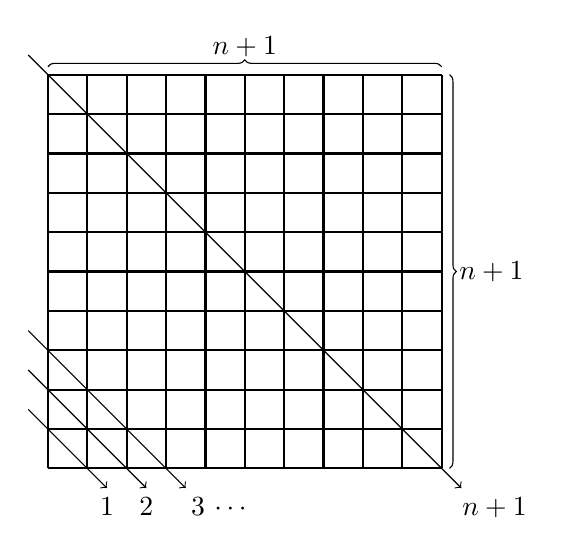
\begin{tikzpicture}[scale=0.5]
		\foreach \r in {0, ..., 10} {
			\draw[black,thick] (0,\r) -- (10,\r);
			\draw[black, thick] (\r,0) -- (\r, 10);
		}
		
		\draw[decoration={brace},decorate]
  			(0,10.2) -- node[above] {$n+1$} (10,10.2);
		\draw[decoration={brace, mirror},decorate]
  			(10.2,0) -- node[right] {$n+1$} (10.2,10);
  			
		\draw[->] (-0.5, 1.5) -- (1.5,-0.5) node[below] {$1$};
		\draw[->] (-0.5, 2.5) -- (2.5,-.5) node[below] {$2$};
		\draw[->] (-0.5, 3.5) -- (3.5,-.5) node[right=12pt, below] {$3$ $\cdots$};
		
		\draw[->] (-0.5, 10.5) -- (10.5,-.5) node[right=12pt, below] {$n+1$};
	
	\end{tikzpicture}
	\end{multicols}
}

\nomen{
	On appelle $S_n$ un \emph{nombre triangulaire} car il apparaît comme le nombre de carrés dans le triangle de la preuve du théorème \ref{thm:triangle}.
}

\notations{
	Au lieu de noter $S_n = 1 + 2 + \cdots + n$, on dit à l'oral « la somme des entiers de 1 à $n$ », car c'est plus court.
	On dit aussi « la somme des $k$, $k$ allant de 1 à $n$ », qu'on choisit de noter
		\[ S_n = 1 + 2 + \cdots + n = \text{« la somme des $k$, $k$ allant de 1 à $n$ »} = \sum_{k=1}^n k, \]
	où la lettre sigma majuscule $\Sigma$ désigne une somme.
	
	Plus généralement, on note
		\[ \sum_{k=a}^b u(k) = u(a) + u(a+1) + \cdots + u(b-1) + u(b). \]
}

\nt{
	Il est également possible d'indexer une somme sur un ensemble.
	Par exemple pour $E=\bigset{7; 11; 13 ; 17}$, 
		\begin{align*}
			\sum_{k\in E} k = 7+11+13+17 = 48, && \text{ et } && \sum_{k\in E} \dfrac1k = \dfrac17+\dfrac1{11}+\dfrac1{13}+\dfrac1{17} \approx 0,3695.
		\end{align*}
	
	Le deuxième théorème de Mertens implique que
		\[ \sum_{p \text{ premier}} \dfrac1p = \pinfty. \]
}

\exe{}{
	Donner les valeurs des sommes suivantes.
	\begin{multicols}{3}
		\begin{enumerate}[label=\roman*)]
		\item
		$\sum\limits_{k=1}^{10} 0$
		
		\item
		$\sum\limits_{k=1}^{10} 1$
		
		\item
		$\sum\limits_{k=0}^{10} 1$
		
		\item
		$\sum\limits_{k=-5}^{11} 1$
		
		\item
		$\sum\limits_{k=4}^{8} 2$
		
		\item
		$\sum\limits_{k=0}^{n} 1$
		
		\item
		$\sum\limits_{k=1}^{10} k$
		
		\item
		$\sum\limits_{k=1}^{20} k$
		
		\item
		$\sum\limits_{k=11}^{20} k$
		\end{enumerate}
	\end{multicols}
}{exe:sommes}{
	\begin{multicols}{3}
		\begin{enumerate}[label=\roman*)]
		\item
		$\sum\limits_{k=1}^{10} 0 = 0$.
		
		\item
		$\sum\limits_{k=1}^{10} 1 = 10$.
		
		\item
		$\sum\limits_{k=0}^{10} 1 = 11$.
		
		\item
		$\sum\limits_{k=-5}^{11} 1 = (11 + 5 + 1) = 17$.
		
		\item
		$\sum\limits_{k=4}^{8} 2 = 2(8-4+1) = 10$.
		
		\item
		$\sum\limits_{k=0}^{n} 1 = n$.
		
		\item
		$\sum\limits_{k=1}^{10} k = \dfrac{10(11)}2 = 55$.
		
		\item
		$\sum\limits_{k=1}^{20} k = \dfrac{20(21)}2 = 210$.
		
		\item
		$\sum\limits_{k=11}^{20} k = \sum\limits_{k=1}^{20} k - \sum\limits_{k=1}^{10} k = 210-55 = 155$.
		\end{enumerate}
	\end{multicols}
}

\thm{Linéarité de la somme}{
	Pour $c\in\R$ et $u, v,$ deux suites, on a 
		\[ \sum_{k=a}^{b} \bigl[ cu(k) + v(k) \bigr] =  c\sum_{k=a}^{b} u(k)+ \sum_{k=a}^{b}v(k). \]
}{thm:linéarité-somme}

\exe{,difficulty=1}{
	Démontrer le théorème \ref{thm:linéarité-somme}.
}{exe:linéarité-somme}{
	En explicitant la somme
		\[ \sum_{k=a}^{b} \bigl[ cu(k) + v(k) \bigr] = cu(a) + v(a) + cu(a+1) + v(a+1) + \cdots + cu(b) + v(b), \]
	on remarque qu'on peut regrouper les termes et factoriser par $c$ pour obtenir
		\[ \sum_{k=a}^{b} \bigl( cu(k) + v(k) \bigr) = c\bigl[u(a) + u(a+1) + \cdots + u(b)\bigr] + \bigl[v(a) + v(a+1) + \cdots + v(b)\bigr] = c\sum_{k=a}^{b} u(k)+ \sum_{k=a}^{b}v(k). \]
}

\lem{}{
	\[ \sum_{k=a}^{b} k = (b-a+1)\dfrac{a+b}2. \]
}{lem:somme-arithm}

\exe{,difficulty=2}{
	Démontrer le lemme \ref{lem:somme-arithm}.
}{exe:lem-somme-arithm}{
	On se ramène au cas $a=0$ pour utiliser le théorème \ref{thm:triangle}.
		\begin{align*}
			\sum_{k=a}^b k = \sum_{k=0}^b k - \sum_{k=0}^{a-1}
								= \dfrac{b(b+1)}2 - \dfrac{a(a-1)}2
								= \dfrac{(a+b)(b-a+1)}2.
		\end{align*}
}

\thm{Somme de série arithmétique}{
	Soit $u$ une suite arithmétique. Alors
		\begin{align*}
			\sum_{k=a}^b u(k) &= \text{(moyenne du premier et dernier terme) $\times$ (nombre de termes)} \\ &= \dfrac{u(a)+u(b)}2 \cdot (b-a+1).
		\end{align*}
}{thm:somme-arithm}

\exe{,difficulty=2}{
	Démontrer le théorème \ref{thm:somme-arithm}.
}{exe:somme-arithm}{
	Posons $u(n) = An +B$.
	Par linéarité de la somme, et d'après le lemme \ref{lem:somme-arithm},
		\begin{align*}
			\sum_{k=a}^b u(k) &= \sum_{k=a}^b \bigl[ Ak + B \bigr], \\
								&= A\sum_{k=a}^b k + B \sum_{k=a}^b 1, \\
								&= A \dfrac{(a+b)(b-a+1)}2 + B(b-a+1), \\
								&= (b-a+1) \dfrac{A(a+b) + 2B}2, \\
								&= (b-a+1) \dfrac{u(a) + u(b)}2.
		\end{align*}
}

\exe{}{
	Montrer que $\sum\limits_{k=a}^b u(k) = \sum\limits_{k=a-1}^{b-1} u(k+1)$.
}{exe:shiftk}{
	Expliciter la somme rend l'identité triviale.
}

\exe{, difficulty=2}{
	Posons $S_n = \sum\limits_{k=1}^{n+1} k^3$. 
	À l'aide de l'exercice \ref{exe:shiftk}, montrer qu'on a
		$S_n = \sum_{k=0}^{n} (k+1)^3.$
	En développant le cube et par linéarité de la somme, montrer que
		\[ S_n = S_n - (n+1)^3 + 3\sum_{k=0}^{n}k^2 + 3\sum_{k=0}^{n}k + n. \]
	En déduire la forme close
		\[ \sum_{k=0}^{n}k^2 = \dfrac{n(n+1)(2n+1)}6. \]
}{exe:somme-carres}{
	TODO
}

\exe{, difficulty=2}{
	En considérant la somme $S_n = \sum\limits_{k=1}^{n+1}k^4$, procéder comme à l'exercice \ref{exe:somme-carres} pour exprimer $\sum\limits_{k=1}^{n+1}k^3$ en fonction de $n$.
	En conclure que 
		\[ (1+2+\cdots+n)^2 = 1^3 + 2^3 + \dots + n^3 = \left[ \dfrac{n(n+1)}2 \right]^2. \]
}{exe:somme-cubes}{
	TODO
}

\exe{}{
	Au regard des exercices \ref{exe:somme-carres} et \ref{exe:somme-cubes}, déterminer combien d'opérations sont nécessaires pour calculer les sommes $1+2^2 + 3^2 + \cdots + n^2$ et $1+2^3 + 3^3 + \cdots + n^3$.
}{exe:complexité-somme}{
	Pour la première, il faut trois multiplications, une division, et deux additions, soit au total 6 opérations.
	Pour la seconde, il faut deux multiplications, une division, et une addition, soit au total 4 opérations.
}

\subsection{Problèmes de seuil}

\section{Suites géométriques}

\subsection{Introduction}

\dfn{Suite géométrique}{
	On dit d'une suite $u$ qu'elle est arithmétique dès qu'elle vérifie, pour tout $n\in\N$,
		\begin{align}\label{eq:suite-geom}
			u(n+1) = q \cdot u(n),
		\end{align}
	où $q \in \R$ est un réel fixé qui ne dépend pas de $n$ appelé la \emph{raison}.
	
	On lit :
		\begin{center}
		« Pour passer d'un terme au suivant, on multiplie par la raison $q$. »
		\end{center}
}{dfn:suite-géométrique}

\mprop{Propriétés des puissances}{
	Soient $a, b, c \in \Z$. On a les relations suivantes.
		\begin{gather*}
			a^{b+c} = a^{b} \times a^{c} \\
			\left(a^b\right)^c = a^{b \times c} \\
			a^{c} \times b^c = \left( a \times b \right)^c
		\end{gather*}
	En particulier, si $a \neq 0$, on a
		\begin{align*}
			a^0 = 1, &
			&a^1 = a, &
			&a^{-1} = \dfrac1a. 
		\end{align*}
}{prop:prop-puissances}

\exe{}{
	Donner les 5 premiers termes de la suite géométrique $u$ de raison 2 et de terme initial $u(0) = 1$.
	Faire une conjecture sur l'expression algébrique de $u(n)$ pour tout $n\in\N$.
}{exe:geom1}{
	Pour passer d'un rang au suivant, on multiplie par la raison, ici $2$.
	Donc $u(1) = 2, u(2) = 4, u(3) = 8, u(4) = 16$.
	
	Il semblerait que $u(n) = 2^n$ pour tout $n\in\N$.
}

\exe{}{
	Montrer que la suite $u$ telle que $u(102) = 25, u(103) = 50, u(104) = 110$ ne peut pas être géométrique.
}{exe:nongeom1}{
	Si $u$ était géométrique, sa raison serait $2$ car c'est ce par quoi on multiplie pour passer du terme 102 au terme 103.
	Cependant, dans ce cas, on aurait $u(104) = 100$, ce qui est contradictoire avec la donnée de l'exercice. \Large\Lightning
}

\exe{}{
	Montrer que la suite $v$ telle que $u(65) = 32, u(67) = 64, u(68) = 128$ ne peut pas être géométrique.
}{exe:nongeom2}{
	Si $v$ était géométrique, sa raison serait $2$ car c'est ce par quoi on multiplie pour passer du terme 67 au terme 68.
	Cependant, dans ce cas, on aurait $u(66) = 32$, et $u(65) = 16$, ce qui est contradictoire avec la donnée de l'exercice. \Large\Lightning
}

\exe{, difficulty=1}{
	Si une suite $w$ vérifie $w(10) = 1, w(11) = 3, w(12) = 9$, est-elle nécessairement géométrique ?
}{exe:nongeom3}{
	$w$ pourrait être géométrique, auquel cas $w(n) = 3^{n-10}$ pour tout $n\in\N$, mais ce n'est pas nécessairement le cas.
	On peut librement définir $w(13) = -10 000$ pour casser le caractère géométrique de la suite. 
}

\exe{}{
	Soit $u$ une suite géométrique de raison $2$ telle que $u(3) = 24$.
	Donner le terme initial de $u$.
}{exe:terme-initial-geom}{
	Pour passer d'un rang au suivant, on doit multiplier par $2$.
	Pour revenir en arrière d'un rang, on multiplie donc par $\dfrac12$.
	Ainsi $u(2) = 24/2 = 12, u(1) = 12/2 = 6$, et $u(0) = 6/2 = 3$.
}


\ex{}{
	La suite $u$ définie par $u(n) = 5 \times 3^n$ pour tout $n\in\N$ est géométrique de raison 3 car
		\begin{align*}
			u(n+1) &= 5 \times 3^{n+1}, \\
					&= 5 \times 3^n \times 3, \\
					&= 3 \times \left( 5 \times 3^n \right), \\
					&= 3 u(n).
		\end{align*}
	Son terme initial est $u(0) = 5 \times 3^0 = 5 \times 1 = 5$.
}{ex:suite-geo}

\exe{}{
	Montrer que la suite $v(n) = 3 \times 2^n$ est géométrique. Donner sa raison et son terme initial.
}{exe:suite-geo}{
	Les propriétés des puissances donnent 
		\begin{align*}
			v(n+1) &= 3 \times 2^{n+1}, \\ 
					&= 3 \times 2 \times 2^n, \\
					&= 2 (3 \times 2^n), \\
					&= 2v(n).
		\end{align*}
	Il suit que $v$ est géométrique de raison 2. Son terme initial est $v(0) = 3$.
}

\subsection{Expression algébrique}

\ex{}{
	Considérons une suite $G$, géométrique de raison $4$ et de terme initial $3$.
	Alors, par définition,
		\[ G(0) = 3. \]
	En spécialisant l'équation \eqref{eq:suite-geom} pour $n=0$, on trouve ensuite
		\[ G(1) = G(0+1) = 4 \times G(0) = 4 \times 3 = 12. \]
	On peut déduire la suite des termes de façon analogue.
		\begin{align*}
			G(0) &= 3 \\
			G(1) &= 4 \times G(0) = 12 \\
			G(2) &= 4 \times G(1) = 48 \\
			G(3) &= 4 \times G(2) = 196 \\
			\vdots &\, \qquad \vdots
		\end{align*}
	On souhaite désormais connaître une formule valable pour tous les entiers naturels $n\in\N$ pour qu'on ait pas à reconstruire la suite depuis le début à chaque étude.
	Pour cela, on choisit de réécrire les termes de la suite de la façon suivante, en utilisant les propriétés de la puissance.
		\begin{align*}
			G(0) &= 3 = 3 \times 4^{0} \\
			G(1) &= 4 \times G(0) = 3 \times 4^{1} \\
			G(2) &= 4 \times G(1) = 3 \times 4^{2} \\
			G(3) &= 4 \times G(2) = 3 \times 4^{3} \\
			\vdots &\, \qquad \vdots \\
			G(n) &= 3 \times 4^n
		\end{align*}
}{}

\thm{de Maya}{
	Soit $v$ une suite géométrique de raison $q \in \R$ et de terme initial $v(0) \in \R$.
	Alors
		\[ v(n) = v(0) \times q^n. \]
}{thm:maya}

\exe{}{
	Pour chacune des suites données algébriquement pour tout $n\in\N$, donner leur raison et leur terme initial.
	\begin{multicols}{2}
	\begin{enumerate}
		\item $u(n) = 2 \times 3^n$
		\item $v(n) = 7 \times \left(\dfrac12 \right)^n$
		\item $\xi(n) = - 6^n$
		\item $a(n) = 11 \times 5^{2n}$
		\item $b(n) = 3 \times 5^{2n+3}$
		\item $c(n) = 10^{-n}$
	\end{enumerate}
	\end{multicols}
}{exe:param-geom}{
	On note $q$ la raison de chacune des suites géométrique.
	Pour une suite géométrique $u$ et par définition, $q = \dfrac{u(1)}{u(0)}$.
	Il suffit donc d'évaluer $u$ en 0 et en 1 pour connaître son terme initial et sa raison lorsqu'elle n'est pas exactement de la forme $u(0) \times q^n$.
	\begin{multicols}{2}
	\begin{enumerate}
		\item $u(0) = 2$ et $q = 3$.
		\item $v(0) = 7$ et $q=\dfrac12$.
		\item $\xi(0) = -1$ et $q=6$.
		\item $a(0) = 11$ et $q = \dfrac{a(1)}{a(0)} = \dfrac{11\times5^2}{11} = 25$.
		\item $b(0) = 3 \times 5^3 = 375$ et $q = \dfrac{b(1)}{b(0)} = \dfrac{3\times5^5}{3\times5^3} = 5^2 = 25$.
		\item $c(0) = 1$ et $q=c(1) = 10^{-1}= \dfrac1{10} = 0,1$.
	\end{enumerate}
	\end{multicols}
}

\exe{, difficulty=1}{
	Considérons la suite $v$ définie par la relation de récurrence suivante, pour tout $n\in\N$.
	\[
	\begin{cases}
		v(0) = 0, \\
		v(n+1) = 2v(n) + 1.
	\end{cases}
	\]
	\begin{enumerate}
		\item Montrer que la suite intermédiaire $w$ définie pour tout $n\in\N$ par
			\[ w(n) = v(n) + 1,\]
		est géométrique.
		\item En déduire que, pour tout $n\in\N$,
			\[ v(n) = 2^n - 1.\]
	\end{enumerate}
}{exe:arithmético-géométrique}{
	Toutes les égalités suivantes sont valables pour tout $n\in\N$.
	\begin{enumerate}
		\item On a $w(n+1) = v(n+1) + 1 = 2v(n) + 1 + 1 = 2\bigl(v(n)+1\bigr) = 2w(n)$.
		$w$ est donc géométrique de raison 2.
		\item De la question précédente, on déduit du terme initial $w(0) = v(0)+1=0+1=1$ que $w(n)=2^n$ grâce au théorème \ref{thm:maya}.
		D'où $v(n) = w(n)-1 = 2^n - 1$.
	\end{enumerate}
}

\subsection{Variations}

\mprop{Variations}{
	Soit $u$ une suite géométrique de raison $q > 0$ et de terme initial $u(0) > 0$.
	On distingue alors les trois cas suivants.
		\begin{enumerate}[label=---]
			\item Si $0 < q < 1$, alors $u$ est décroissante et tend vers $0$ exponentiellement.
			\item Si $q=1$, alors $u$ est constante : $u(n) = u(0)$ pour tout $n\in\N$.
			\item Si $q>1$, alors $u$ est croissante et diverge exponentiellement vers $+ \infty$.
		\end{enumerate}
}{}

\subsection{Sommes}

\thm{}{
	Pour tout $n\in\N$, on a l'égalité
		\[ 1 + q + q^2 + \cdots + q^n  = \dfrac{1-q^{n+1}}{1-q}. \]
}{thm:somme-geom}
\pf{}{
	Somme téléscopique.
}

\exe{, difficulty=2}{
	On souhaite étudier la série de Bâle\footnotemark $S_n = \sum\limits_{k=1}^n \dfrac{1}{k^2}$. 
	En particulier on se demande si $S_n$ diverge ou si elle est bornée supérieurement. 
	
	Montrer que $\dfrac1{k(k+1)} = \dfrac1k - \dfrac1{k+1}$ pour tout $k\geq1$
	et en déduire que, pour tout $n\in\N$,
		\[ \sum_{k=1}^n \dfrac1{k(k+1)} = 1 - \dfrac1{n+1}. \]
	Pour tout $k, n \in\N$, montrer que $k(k+1) \geq (k+1)^2$ et conclure que $S_n \leq 2-\dfrac1n \leq 2$.
}{exe:serie-bale}{
	TODO
}
\footnotetext{Notamment étudiée par Jacques Bernoulli (165?-1705), mathématicien et physicien suisse né à Bâle.}

\nt{
	Euler\footnotemark démontra (plus ou moins rigoureusement) en 1735 que
		\[ \sum_{k=1}^{\infty} \dfrac1k = \dfrac{\pi^2}6. \]
}
\footnotetext{Leonhard Euler (1707-1783), mathématicien et physicien suisse né à Bâle.}

\subsection{Problèmes de seuil}

\str{
	On décrit ici une stratégie pour résoudre un problème de seuil courant qui est facile à résoudre pour les suites arithmétiques mais très dur à résoudre pour les suites géométriques.
	Étant donné une suite géométrique $v$ croissante et un seuil $M > 0$, on souhaite trouver le plus petit entier naturel $N\in\N$ vérifiant
		\[ v(N) > M. \]
	Considérons l'exemple suivant.
		\begin{align*}
			v(n) = 3 \times 5^n && \text{et} && M = 100~000.
		\end{align*}
	La stratégie est de considérer un intervalle dans lequel le $N$ recherché doit nécessairement appartenir, et de scinder cet intervalle à chaque étape.
	Pour commencer, on prend
		\[ I = [0 ; 10], \]
	car $v(0) = 3 < 100~000 < v(10) \approx 2,9 \times 10^{7}$.
	La borne supérieure $10$ a été choisie au hasard et suffisamment grande telle que $v(10)$ dépasse le seuil.
	
	On divise l'intervalle en deux parts égales en considérant son milieu, 
		\[ m = \dfrac{0+10}2 = 5. \]
	On évalue $v$ en $5$ pour décider si $N$ est plus grand ou plus petit que $5$.
	En l'occurrence, 
		\[ v(5) = 9375 < 100~000. \]
	Le seuil recherché est donc nécessairement supérieur à $5$, et on peut définir
		\[ I = [5 ; 10], \]
	comme nouvel intervalle dans lequel $N$ appartient.
	
	On répète l'opération en calculant le milieu $m = \dfrac{5+10}2 = 7,5$, et 
		\[ v(7,5) \approx 5,2 \times 10^5 > 100~000. \]
	D'où $I = [5 ; 7,5]$.
	Ici, on peut soit tester les $3$ valeurs qui restent ($5 ; 6 ; 7$) ou continuer pour trouver
		\[ I = [ 6,25 ; 7,5 ], \]
	dans lequel $N = 7$ est le seul entier possible.
	
	On vérifiera bien sûr que $v(6) < 100~000 < v(7)$, comme voulu.
}{}

\IncMargin{1em}
\begin{algorithm}
\SetKwInput{KwRes}{retourner}%
\SetKwIF{Si}{SinonSi}{Sinon}{si}{alors}{sinon si}{sinon}{fin si}%
\SetKwFor{Tq}{tant que}{faire}{fin tq}%
\SetKwInOut{Input}{entrée}\SetKwInOut{Output}{sortie}
	\Input{Suite géométrique $G$ de raison $q > 1$ tel que $G(0) > 0$. Seuil $M$. Intervalle $I=[a ; b]$ tel que $G(a) < M < G(b)$.}
	\Output{Le plus petit entier naturel $N\in\N$ tel que $G(N) \geq M$.}
	\BlankLine
	\emph{L'intervalle $I=[a;b]$ de départ doit vérifier $G(a) < M < G(b)$, de telle sorte que l'entier $N$ recherché lui appartienne nécessairement car $G$ est croissante. On pourrait prendre $a=0$ et $b$ extrêmement grand en cas de doute.}\\
	\Tq{ la longueur de l'intervalle $I=[a;b]$ est supérieure  ou égale à $1$}{
		$m = \dfrac{a+b}2$ \emph{, le milieu de l'intervalle $I$}\\
		\Si{ $G(m) \geq M$}{
			$I = [a ; m]$
		}
		\Sinon{
			$I = [m ; b]$
		}
	}
	\KwRes{L'unique entier appartenant à l'intervalle $I$.}
\caption{Problème de seuil.}\label{algo:seuil-geom}
\label{alg:seul-geom}
\end{algorithm}\DecMargin{1em} 

\nt{
	C'est au début du 17è siècle que John Neper crée les premières tables de valeurs de la fonction $\ln$ qui porte son nom : le logarithme népérien.
	La notation $\log$ désigne une fonction qui transforme la multiplication en une addition, cette dernière opération étant beaucoup plus facile lorsqu'on manipule des grands nombres.
	Une bonne table de valeurs permet alors, pour multiplier deux grands nombres $A$ et $B$, d'additionner leur logarithmes grâce à la relation
		\[ \log(A \times B) = \log(A) + \log(B). \]
	Pour retrouver le produit, on utilise alors la table de valeurs dans le sens inverse.
	
	Plus généralement, l'application du $\log$ convertit une équation exponentielle en une équation linéaire simple.
}{}

\subsection{Échelle logarithmique}


\section{Implémentation}

\exe{}{
	On appelle $H_n = \sum\limits_{k=1}^n \dfrac1k$ la \emph{série harmonique}.
	Implémenter la fonction $H_n$ et donner la valeur approximative de $H_{100}$.
	Ensuite, trouver le premier rang $n$ vérifiant $H_n \geq 10$.
}{exe:serie-harmonique}{
	Voici deux implémentation de $H_n$ possibles. On obtient $H_{100} \approx 5,1873$.

	\begin{multicols}{2}
	\python{harmonic-series}
	\columnbreak
	\python{harmonic-series-2}
	\end{multicols}
}

\exe{}{
	Trouver le premier rang $n$ vérifiant $H_n \geq 10$, où $H_n$ désigne la série harmonique définie à l'exercice \ref{exe:serie-harmonique}.
}{exe:seuil-harmonique}{
	Voici une implémentation permettant de trouver le premier rang $n$ vérifiant $H_n \geq 10$. On obtient $n=12369$.
	
	\python{harmonic-series-3}
}



\exe{}{
	Implémenter l'algorithme \ref{alg:seul-geom} et trouver le plus petit entier naturel $n\in\N$ vérifiant les inéquations suivantes.
	\begin{multicols}{2}
	\begin{enumerate}
		\item $2 \times 3^n > 100~000$
		\item $7 \times \left(\dfrac32 \right)^n > 50~000$
		\item $3 \times \left( \dfrac43 \right)^n > 1~000$
		\item $3 \times \left( \dfrac43 \right)^n > 10~000$
	\end{enumerate}
	\end{multicols}
}{}


